\section{The Chromatic Number Problem}\label{sec:chromatic}

The chromatic number problem is \emph{inherently intractable}.  Informally, this means that finding a solution for
a given input graph, regardless of the means, can take a very, very long time in the worst cases.  Thus, trying to
find an efficient but exact method of solution that satisfies all cases is a fool's errand; about the best that can
be done is to perform better than existing well-known methods in most cases.  This section begins with a brief
overview of inherent intractability and describes why the chromatic number problem is of this type.  Most of this
material is based on the early yet still very influential text by Garey and Johnson (1979)~\cite{garey} with some
help from Spiser (2013)~\cite{sipser}.  Following the overview is an examination of some of the well-known
algorithms for finding the chromatic number of a graph.

\subsection{Problems}\label{sec:sub:problems}

A \emph{problem} consists of three parts:

\begin{enumerate}
\item A specific question to be answered.
\item A description of zero or more input \emph{parameters}.
\item A statement of the properties that the \emph{solution} is required to satisfy.
\end{enumerate}

An \emph{instance} of a problem is constructed by specifying particular values for each input parameter.  The
step-by-step procedure that translates the input parameters to a corresponding well-defined solution is called an
\emph{algorithm}.  To say that an algorithm \emph{solves} a problem \(\Pi\) means that the algorithm produces a
valid solution for every possible instance \(I\) of the problem \(\Pi\).

The chromatic number problem accepts a graph \(G\) and uses an algorithm to obtain a number \(k\in\N\) where \(k\)
is the minimum value such that \(G\) is \colorable{k}.  The proposed algorithm is one such algorithm that can be
used to solve the problem.  Other examples are the Christofides (1971)~\cite{christofides} and the Corneil/Graham
(1973)~\cite{corneil} algorithms, which are introduced later in this section and will be compared to the proposed
algorithm using random graph analysis.

\subsection{Comparing Algorithms}\label{sec:sub:compare}

Computation theory is the branch of computer science that is concerned with determining and comparing the runtime
performance of algorithms.  The history and specifics of computation theory, although interesting, are beyond the
scope of this research.  This section presents a brief overview of what is needed from the field of computation
theory in order to characterize the chromatic number problem.

Algorithms are typically compared using three parameters:
\begin{enumerate}
\item Runtime complexity
\item Space complexity
\item Runtime duration
\end{enumerate}

These parameters are discussed in the following sections.

\subsubsection{Runtime Complexity}\label{sec:sub:sub:runtime}

\emph{Runtime complexity} measures the number of \emph{steps} required to obtain a solution for the worst possible
input parameter and is a function of some \emph{length} parameter of the problem.  For graph algorithms, the length
parameter is usually the order of the graph, although size and structure can also affect the worst case scenario.

The runtime complexity of an algorithm is stated using the so-called \emph{big-\(\BO\)} notation: to say that an
algorithm has \(\BO(f(n))\) runtime complexity means that the maximum number of steps required to obtain a solution
for a given length parameter \(n\) is asymptotic to the function \(f(n)\) as \(n\to\infty\).  Roughly speaking,
tractable problems are those problems with polynomial \(\BO(n^c)\) or better runtime complexity for some real
number constant \(c\ge0\), and intractable problems are those problems with exponential \(\BO(c^{f(n)})\) or worse
runtime complexity for some real number constant \(c>1\).  Exponential problems are usually associated with
so-called \emph{brute force} algorithms that must try all possibilities from an exponentially increasing set of
candidate solutions in order to find the desired solution.

What constitutes a \emph{step} in an algorithm is relative to the overall runtime complexity of the algorithm: any
process that has significantly less runtime complexity than the runtime complexity of the whole algorithm can be
called a step.  For example, a process that has polynomial runtime complexity can be called a step of an algorithm
that has exponential runtime complexity.

Runtime complexity is used in two different ways to compare algorithms:
\begin{enumerate}
\item What is the runtime complexity for finding a solution to a problem given a particular input parameter?
\item What is the runtime complexity for verifying that a given solution is in fact a solution for a given
  input parameter?
\end{enumerate}

The two comparisons can be very different.  For example, finding a \clique{k} in a graph \(G\) for a particular value
of \(k\) has exponential runtime complexity; however, determining whether or not a given subgraph of a graph is a
\(k\)-clique has polynomial runtime complexity.

These two methods of comparison are used to classify the runtime complexity of algorithms as follows:
\begin{description}
\item[P] Algorithms with polynomial or better runtime complexity to find or verify a solution.
\item[NP] A superset of P with varying runtime complexity to find a solution but polynomial runtime complexity to
  verify a solution.
\item[NP-complete] A subset of NP problems that have been proven to have the same runtime complexity to find a
  solution.  It is an open question as to whether \(P=NP\); however, it is conjectured that they are not equal.
\item[NP-hard] Algorithms that have been proved to have the same runtime complexity as the NP-complete problems to
  find a solution but varying runtime complexity to verify a solution.
\end{description}

The relationships between these runtime complexity classes, assuming \(P\ne NP\), is shown in
\figurename~\ref{fig:complexity}.

\begin{figure}[H]
  \centering
  \begin{tikzpicture}
    \node at (0,0) [circle,draw,minimum size=2in] {NP};
    \node at (0,-1.5) [ellipse,draw,minimum width=1in, minimum height=0.5in] {P};
    \draw (0,1) parabola (3,4);
    \draw (0,1) parabola (-3,4);
    \node at (0,1.75) {NP-complete};
    \node at (0,3.25) {NP-hard};
  \end{tikzpicture}
  \caption{The runtime complexity classes.}
  \label{fig:complexity}
\end{figure}

For the purposes of this research, the NP-complete problems are assumed to have exponential runtime complexity to
find a solution and polynomial runtime complexity to verify a solution, and the NP-hard problems are assumed to
have exponential runtime for both finding and verifying solutions.

The chromatic number problem is NP-hard: it requires exponential time to exhaustively generate and check all
possible independent set partitions to find a partition with the smallest number of independent sets \(k\), and the
same basic procedure must be used to verify that given a supposed \(k\)-chromatic coloring, there does not exist a
proper coloring for smaller \(k\).

\subsubsection{Space Complexity}\label{sec:sub:sub:space}

\emph{Space complexity} measures the maximum amount of memory required at any point in time when an algorithm is
run on a computer program.  The limited memory and CPU power in early computers forced algorithm designers and
programmers to make careful tradeoffs between CPU cycles and the storage of intermediate results.  With today's
fast CPUs and practically unlimited virtual memory systems, such concerns are not as important.  Thus, space
complexity will not be considered when comparing the selected well-known algorithms to the proposed algorithm.

\subsubsection{Runtime Duration}\label{sec:sub:sub:duration}

\emph{Runtime duration} is an empirical measurement of how long an algorithm runs on a given computer, usually on
best, average, and worst-case input parameter values.  Determining the runtime complexity for some algorithms can
be very complicated when the number of possible steps is dependent on the peculiarities of the input parameters.
In the case of graph algorithms, such things as order, size, and edge density can all affect the number of steps.
Furthermore, runtime complexity is geared towards theoretical comparisons between algorithms, not actual runtime of
an algorithm implementation on a given computer.  Thus, an important part of this research is a random graph
analysis of several well-known algorithms and the proposed algorithm.

\subsection{Estimating the Chromatic Number of a Graph}

Since the chromatic number problem is NP-hard, an alternative to finding an exact answer is to find lower and upper
bounds for the actual value.  If these bounds happen to match then they provide the actual chromatic number.  The
following sections describe well-known methods for finding the upper and lower bounds for the chromatic number of a
graph.

\subsubsection{Finding a Lower Bound}\label{sec:sub:sub:lower}

\subsubsection{Finding an Upper Bound}\label{sec:sub:sub:upper}

\subsection{The Christofides Algorithm}\label{sec:sub:christofides}

\subsection{Zykov Algorithms}\label{sec:sub:zykov}

An exhaustive, exponential-time algorithm for determining the chromatic number of a graph is derived from a
nondeterministic Turing machine technique attributed to Ukranian graph theorist Alexandre A. Zykov (1922--2013)
\cite{obit}.

\begin{figure}[h]
  \label{fig:zykov}
  \begin{center}
    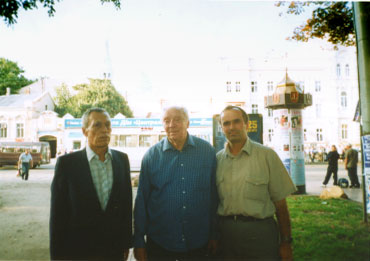
\includegraphics{zykov}
  \end{center}
  \caption{V.G Vizing (L), A.A. Zykov (C), and V.I. Voloshin (R) in Odessa (2001) \cite{voloshin}}
\end{figure}

\subsubsection{The Chromatic Polynomial}

In his 1949 paper (translated by the AMS in 1952) \cite{zykov}, Zykov addresses the question: given a graph \(G\) and
a number \(k\in\N\), how many ways are there to properly color \(G\) using at most \(k\) colors?  In fact, he is not
particularly concerned about the chromatic number, which he calls the \emph{rank}, of a graph.  To solve this problem,
Zykov notes that in any proper coloring of a graph:
\begin{enumerate}
\item Nonadjacent vertices have either the same color or different colors.
\item Adjacent vertices always have different colors.
\end{enumerate}
If nonadjacent vertices have the same color then they can be contracted and the resulting graph retains the same
\coloring{k} as the original graph.  This is demonstrated in Figure \ref{fig:zvcon}.

\begin{figure}[h]
  \label{fig:zvcon}
  \begin{center}
    \begin{minipage}{2in}
      \begin{center}
        \begin{tikzpicture}[every node/.style={labeled node}]
          \colorlet{c1}{green!25!white}
          \colorlet{c2}{blue!25!white}
          \colorlet{c3}{red!25!white}
          \node (d) [fill=c2] at (0,0) {\(d\)};
          \node (c) [fill=c3,right=of d] {\(c\)};
          \node (b) [fill=c2,above=of c] {\(b\)};
          \node (a) [fill=c1,above=of d] {\(a\)};
          \draw (a) -- (b);
          \draw (a) -- (c) -- (d) -- (a);
        \end{tikzpicture}

        \bigskip

        \(G\)
      \end{center}
    \end{minipage}
    \begin{minipage}{2in}
      \begin{center}
        \begin{tikzpicture}[every node/.style={labeled node}]
          \colorlet{c1}{green!25!white}
          \colorlet{c2}{blue!25!white}
          \colorlet{c3}{red!25!white}
          \node (bd) [fill=c2] at (0,0) {\(bd\)};
          \node (c) [fill=c3,right=of bd] {\(c\)};
          \node (a) [fill=c1,above=of bd] {\(a\)};
          \draw (a) -- (c) -- (bd) -- (a);
        \end{tikzpicture}

        \bigskip

        \(G\cdot bd\)
      \end{center}
    \end{minipage}
  \end{center}
  \caption{Same Colors with Vertex Contraction}
\end{figure}

If nonadjacent vertices have different colors then they can be joined by an edge and the resulting graph retains
the same \coloring{k} as the original graph.  This is demonstrated in Figure \ref{fig:zeadd}.

\begin{figure}[h]
  \label{fig:zeadd}
  \begin{center}
    \begin{minipage}{2in}
      \begin{center}
        \begin{tikzpicture}[every node/.style={labeled node}]
          \colorlet{c1}{green!25!white}
          \colorlet{c2}{blue!25!white}
          \colorlet{c3}{red!25!white}
          \node (d) [fill=c2] at (0,0) {\(d\)};
          \node (c) [fill=c3,right=of d] {\(c\)};
          \node (b) [fill=c2,above=of c] {\(b\)};
          \node (a) [fill=c1,above=of d] {\(a\)};
          \draw (a) -- (b);
          \draw (a) -- (c) -- (d) -- (a);
        \end{tikzpicture}

        \bigskip

        \(G\)
      \end{center}
    \end{minipage}
    \begin{minipage}{2in}
      \begin{center}
        \begin{tikzpicture}[every node/.style={labeled node}]
          \colorlet{c1}{green!25!white}
          \colorlet{c2}{blue!25!white}
          \colorlet{c3}{red!25!white}
          \node (d) [fill=c2] at (0,0) {\(d\)};
          \node (c) [fill=c3,right=of d] {\(c\)};
          \node (b) [fill=c2,above=of c] {\(b\)};
          \node (a) [fill=c1,above=of d] {\(a\)};
          \draw (a) -- (b) -- (c);
          \draw (a) -- (c) -- (d) -- (a);
        \end{tikzpicture}

        \bigskip

        \(G+bc\)
      \end{center}
    \end{minipage}
  \end{center}
  \caption{Different Colors with Edge Addition}
\end{figure}

By applying these steps recursively, all of the possible distributions of the nonadjacent nodes to independent sets
are generated.  The termination condition for each recursive path is a complete graph of some varying order \(k\).
Each node in the complete graph represents an independent set of nonadjacent nodes in the original graph that have
been combined via vertex contraction.  Thus, each complete graph of order \(k\) represents a possible \coloring{k}
of the original graph.  The complete graphs of smallest order represent chromatic colorings and their order is the
chromatic number of the original graph.

Zykov uses a graph equation syntax to record the recursive processing of a graph, where each line in the equation
represents the next recursive layer.  Isomorphic graphs are combined with a frequency multiplier at each layer.
This is demonstrated in Figure \ref{fig:greqn}.

\begin{figure}[h]
  \label{fig:greqn}
  \begin{align*}
    \begin{minipage}{0.75in}
      \begin{center}
        \begin{tikzpicture}[every node/.style={unlabeled node}]
          \node (a1) at (0,0) {};
          \node (a2) [right=of a1] {};
          \node (a3) [above=of a2] {};
          \node (a4) [above=of a1] {};
          \draw (a3) -- (a4) -- (a1) -- (a2) -- (a4);
        \end{tikzpicture}
      \end{center}
    \end{minipage} &=
    \begin{minipage}{0.75in}
      \begin{center} 
        \begin{tikzpicture}[every node/.style={unlabeled node}]
          \node (b1) at (0,0) {};
          \node (b2) [above=of b1] {};
          \node (b3) [right=of b1] {};
          \draw (b1) -- (b2) -- (b3) -- (b1);
        \end{tikzpicture}
      \end{center}
    \end{minipage} +
    \begin{minipage}{0.75in}
      \begin{center}
        \begin{tikzpicture}[every node/.style={unlabeled node}]
          \node (c1) at (0,0) {};
          \node (c2) [right=of a1] {};
          \node (c3) [above=of a2] {};
          \node (c4) [above=of a1] {};
          \draw (c2) -- (c3) -- (c4) -- (c1) -- (c2) -- (c4);
        \end{tikzpicture}
      \end{center}
    \end{minipage} \\
    &= \begin{minipage}{0.75in}
      \begin{center} 
        \begin{tikzpicture}[every node/.style={unlabeled node}]
          \node (b1) at (0,0) {};
          \node (b2) [above=of b1] {};
          \node (b3) [right=of b1] {};
          \draw (b1) -- (b2) -- (b3) -- (b1);
        \end{tikzpicture}
      \end{center}
    \end{minipage} +
    \begin{minipage}{0.75in}
      \begin{center} 
        \begin{tikzpicture}[every node/.style={unlabeled node}]
          \node (b1) at (0,0) {};
          \node (b2) [above=of b1] {};
          \node (b3) [right=of b1] {};
          \draw (b1) -- (b2) -- (b3) -- (b1);
        \end{tikzpicture}
      \end{center}
    \end{minipage} +
    \begin{minipage}{0.75in}
      \begin{center}
        \begin{tikzpicture}[every node/.style={unlabeled node}]
          \node (c1) at (0,0) {};
          \node (c2) [right=of a1] {};
          \node (c3) [above=of a2] {};
          \node (c4) [above=of a1] {};
          \draw (c2) -- (c3) -- (c4) -- (c1) -- (c2) -- (c4);
          \draw (c1) -- (c3);
        \end{tikzpicture}
      \end{center}
    \end{minipage} \\
    &= 2
    \begin{minipage}{0.75in}
      \begin{center} 
        \begin{tikzpicture}[every node/.style={unlabeled node}]
          \node (b1) at (0,0) {};
          \node (b2) [above=of b1] {};
          \node (b3) [right=of b1] {};
          \draw (b1) -- (b2) -- (b3) -- (b1);
        \end{tikzpicture}
      \end{center}
    \end{minipage} +
    \begin{minipage}{0.75in}
      \begin{center}
        \begin{tikzpicture}[every node/.style={unlabeled node}]
          \node (c1) at (0,0) {};
          \node (c2) [right=of a1] {};
          \node (c3) [above=of a2] {};
          \node (c4) [above=of a1] {};
          \draw (c2) -- (c3) -- (c4) -- (c1) -- (c2) -- (c4);
          \draw (c1) -- (c3);
        \end{tikzpicture}
      \end{center}
    \end{minipage} \\
    &= 2K_3+K_4
  \end{align*}
  \caption{Zykov Graph Equation}
\end{figure}

Determining whether two graphs are isomorphic is hard, so combining isomorphic graphs in all but the very simple
cases should be skipped; the complete graphs resulting from the further processing of two isomorphic graphs will
eventually be combined anyway by the end.

Zykov was trying to determine the number of \coloring{k}s of a graph without color indifference: each permutation
of colors for a particular distribution is considered unique.  Thus, Zykov multiplied each complete graph
coefficient in the final line of a graph equation by the number of permutations from selecting the order \(n\) of
the particular complete graph from \(k\) colors:
\[k^{(n)}=k(k-1)(k-2)\cdots(k-n+1)\]
Thus, the total number of unique colorings from the example shown in Figure \ref{fig:greqn} using \(k\) colors
would be:
\[M(G,k)=2k^{(3)}+k^{(4)}\]
This is known as the factorial form of the \emph{chromatic polynomial} for the graph.  The corresponding
\emph{expanded form} is:
\[M(G,k)=k^4-4k^3+5k^2-2k\]
Read (1968) \cite{read} expands on the construction of the factorial form of the chromatic polynomial for a graph
and proves several theorems regarding the expanded form.  Some examples are:
\begin{enumerate}
\item \(M(G,k)=M(G\cdot uv)+M(G+uv)\), where \(u\) and \(v\) are any two nonadjacent vertices in the current
  recursive step.
\item The degree of M(G,k) is the order of \(G\).
\item The highest order coefficient is \(1\).
\item There is no constant term.
\item The terms alternate in sign.
\end{enumerate}
In fact, Read shows that the expanded form is actually an inclusion-exclusion equation resulting from starting with
all possible proper and improper colorings \(k^n\) and then subtracting the improper colorings.

\subsubsection{An Exhaustive Algorithm}

Corneil and Graham extend Zykov's work with the following theorem \cite{corneil}:

\begin{theorem}[Corneil and Graham, 1973]
  \label{thm:corneil}
  Let \(G\) be a graph and let \(u\) and \(v\) be two nonadjacent vertices in \(G\):
  \[\X(G)=\min\set{\X(G\cdot uv),\X(G+uv)}\]
\end{theorem}

Zykov's method combined with Theorem \ref{thm:corneil} can be used to construct an exhaustive algorithm for finding
the chromatic number and a chromatic coloring for a graph \(G\).  We define \(S\) to be a first-in-first out (FIFO)
stack of graphs and \(X\) to be the last found complete graph of the smallest order.  Each vertex in \(X\)
represents a set of contracted vertices.
\begin{enumerate}
\item Construct a graph \(G'\) that is isomorphic to \(G\) and where each vertex in \(G'\) is a list of contracted
  vertices initialized to a one element list containing the corresponding vertex in \(G\).
\item Push \(G'\) onto \(S\).
\item \label{step:zempty} If \(S\) is empty then return \(n(X)\) and \(X\).
\item \label{step:zcheck} If the graph on the top of \(S\) is complete:
  \begin{enumerate}
  \item Pop the graph off of the top of \(S\) and save it as \(H\).
  \item If \(X\) is not set or \(n(H)<n(X)\) then let \(X=H\).  Otherwise, discard \(H\).
  \item Go to step \ref{step:zempty}.
  \end{enumerate}
\item The graph on the top of \(S\) is not complete.  Pop the graph off of \(S\) and save it as \(H\).
\item Pick any two nonadjacent vertices \(u\) and \(v\) in \(H\).
\item Push \(H+uv\) onto \(S\).
\item Construct \(H'=H\cdot uv\), where the contracted vertex list for the new contracted vertex is a concatenation
  of the lists for \(u\) and \(v\).
\item Push \(H'\) onto \(S\).
\item Go to step \ref{step:zcheck}.
\end{enumerate}

The steps of this algorithm can be tracked via a so-called \emph{Zykov tree} \cite{corneil}.  The Zykov tree for
the example in Figure \ref{fig:greqn} is shown in Figure \ref{fig:ztree}.  Note that the exhaustive algorithm
corresponds to a depth-first walk of the tree.

\begin{figure}[h]
  \label{fig:ztree}
  \begin{center}
    \begin{tikzpicture}
      \node (a) [draw,circle] at (0,0) {
        \begin{tikzpicture}[every node/.style={unlabeled node}]
          \node (a1) at (0,0) {};
          \node (a2) [right=of a1] {};
          \node (a3) [above=of a2] {};
          \node (a4) [above=of a1] {};
          \draw (a3) -- (a4) -- (a1) -- (a2) -- (a4);
        \end{tikzpicture}
      };
      \node (b) [draw,circle,below left=of a] {
        \begin{tikzpicture}[every node/.style={unlabeled node}]
          \node (b1) at (0,0) {};
          \node (b2) [above=of b1] {};
          \node (b3) [right=of b1] {};
          \draw (b1) -- (b2) -- (b3) -- (b1);
        \end{tikzpicture}
      };
      \node (c) [draw,circle,below right=of a] {
        \begin{tikzpicture}[every node/.style={unlabeled node}]
          \node (c1) at (0,0) {};
          \node (c2) [right=of a1] {};
          \node (c3) [above=of a2] {};
          \node (c4) [above=of a1] {};
          \draw (c2) -- (c3) -- (c4) -- (c1) -- (c2) -- (c4);
        \end{tikzpicture}
      };
      \node (d) [draw,circle,below left=of c] {
        \begin{tikzpicture}[every node/.style={unlabeled node}]
          \node (d1) at (0,0) {};
          \node (d2) [above=of d1] {};
          \node (d3) [right=of d1] {};
          \draw (d1) -- (d2) -- (d3) -- (d1);
        \end{tikzpicture}
      };
      \node (e) [draw,circle,below right=of c] {
        \begin{tikzpicture}[every node/.style={unlabeled node}]
          \node (c1) at (0,0) {};
          \node (c2) [right=of a1] {};
          \node (c3) [above=of a2] {};
          \node (c4) [above=of a1] {};
          \draw (c2) -- (c3) -- (c4) -- (c1) -- (c2) -- (c4);
          \draw (c1) -- (c3);
        \end{tikzpicture}
      };
      \draw (a) edge (b) edge (c);
      \draw (c) edge (d) edge (e);
    \end{tikzpicture}
  \end{center}
  \caption{A Zykov Tree}
\end{figure}

\subsubsection{Branch and Bound Strategies}

Using a Zykov tree suggests that the exhaustive algorithm is a candidate for a branch-and-bound solution, where the
branching is accomplished via vertex contraction and edge addition and the bounding is some method to prematurely
terminate a branch.  Corneil and Graham suggest such a bounding technique through the determination of so-called
\(\a\)-clusters; however, the algorithm for finding such clusters has \(\BO(n^3)\) runtime complexity.
